\section*{Overview}

This report documents the implementation of Parts A (Data Management Backbone) and C (Orchestration Framework) of Lab 3. Our solution implements a comprehensive data lake architecture using PySpark 4.0, Delta Lake, MLFlow, and Apache Airflow 3.0 to process Barcelona's Open Data for real estate and socioeconomic analysis. All outputs are bundled in a comprehensive Streamlit application, providing an interface to our services and analysis (cf. \verb|README.md|). In the following, we sketch our data pipelines (cf. \figureref{fig:pipe_abs}):

\begin{figure}[H]
    \centering
    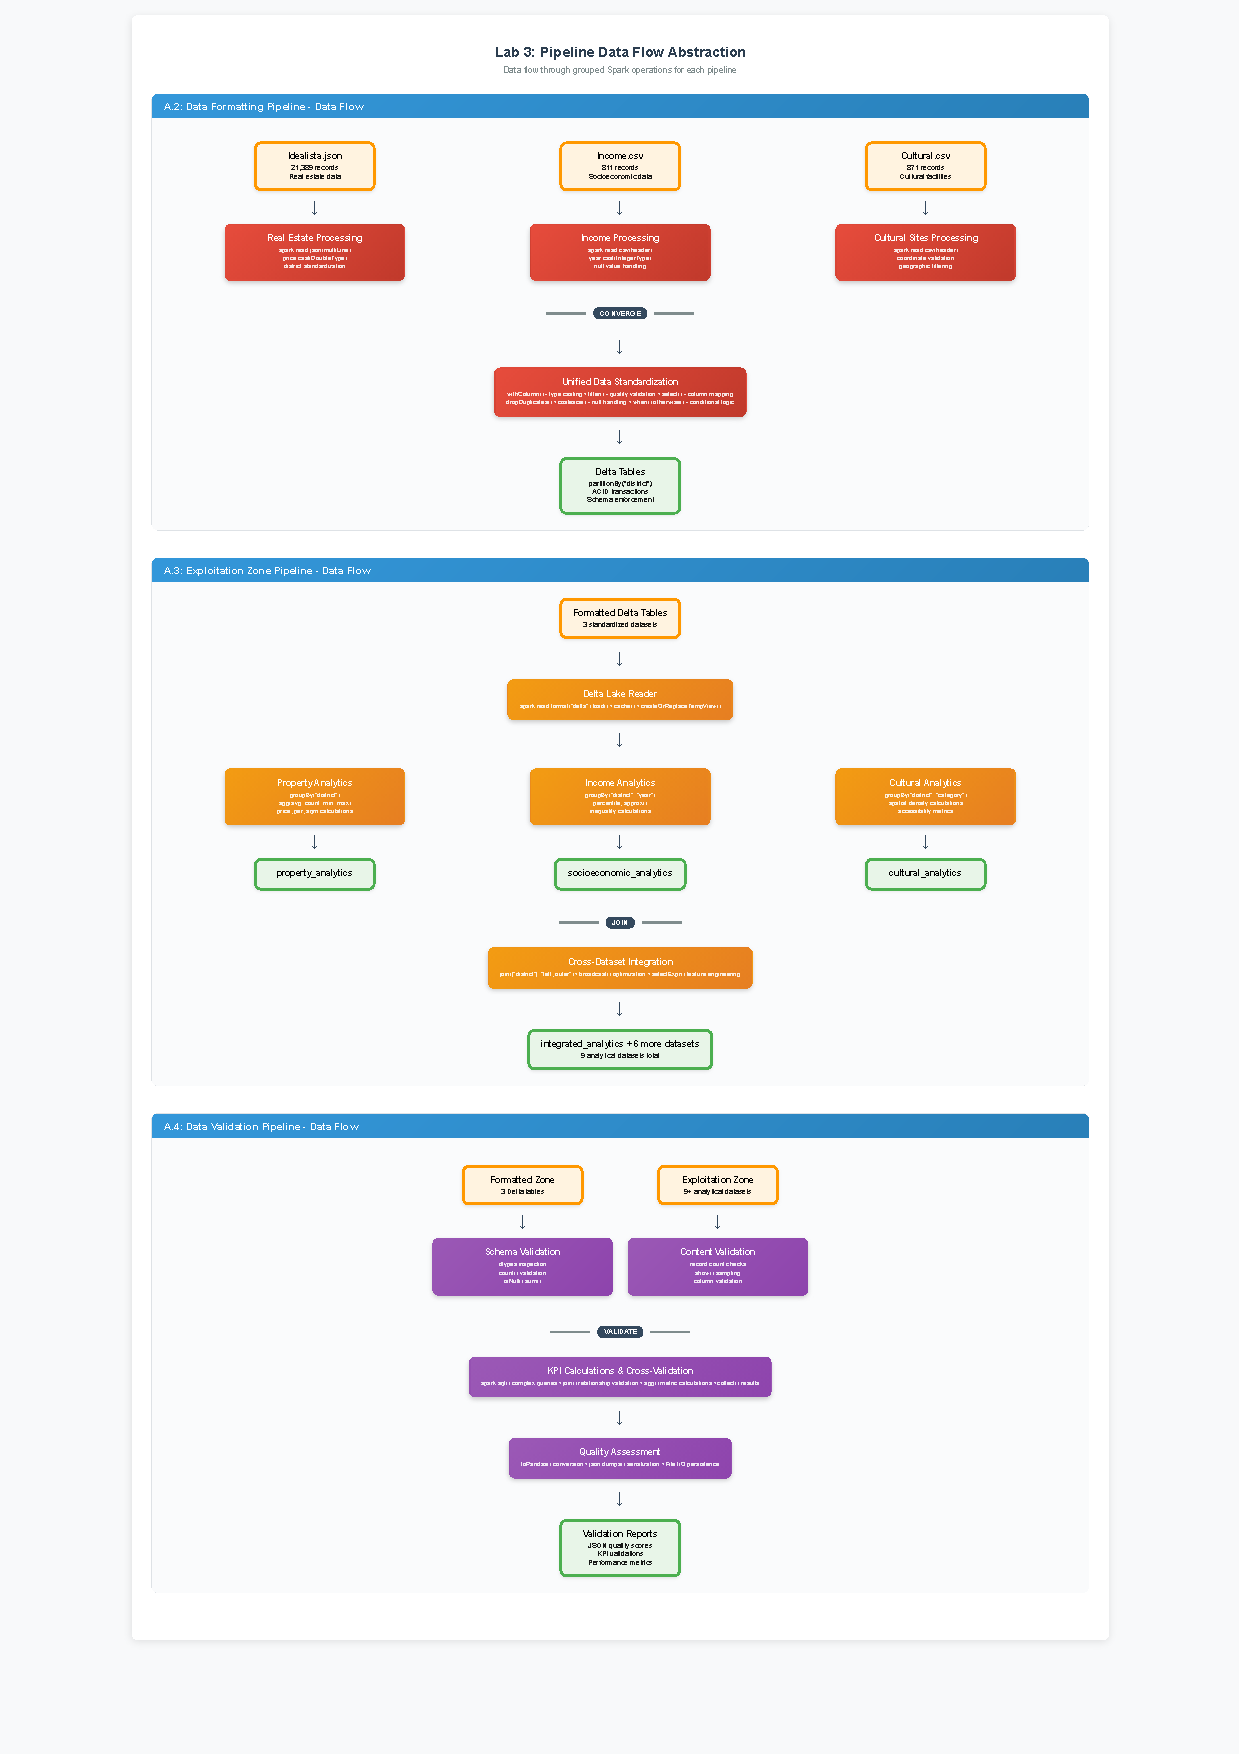
\includegraphics[width=.8\linewidth]{latex/imgs/pipeline_abstraction.pdf}
    \caption{Abstract pipeline sketch}
    \label{fig:pipe_abs}
\end{figure}

\section{Data Management Backbone}

\subsection{Dataset Selection \& KPI Definition}

We selected three datasets from Barcelona's Open Data portal, satisfying all requirements:

\begin{itemize}[nosep]
\item \textbf{Idealista} (JSON, 21,389 records): Real estate listings with comprehensive property characteristics, prices, and geographic coordinates
\item \textbf{Income} (CSV, 811 records): Socioeconomic data by district/neighborhood (2007-2017) with excellent data quality (0\% missing)
\item \textbf{Cultural Sites} (CSV, 871 records): Geographic distribution of cultural amenities across Barcelona
\end{itemize}

Our analysis focuses on \textbf{10 comprehensive KPIs} spanning housing affordability, socioeconomic equity, and urban quality of life, including Housing Affordability Ratio, Income Inequality Index, Cultural Density, and Neighborhood Attractiveness Score.

\subsection{Data Formatting Pipeline}

\textbf{Implementation:} \texttt{src/airflow/dags/pipelines/a2.py}

The formatting pipeline transforms raw data from Landing Zone into standardized Delta tables:

\begin{itemize}[nosep]
\item \textbf{Data Standardization:} Schema unification, data type casting, and column naming conventions
\item \textbf{Quality Enhancement:} Duplicate removal, missing value imputation, and outlier detection
\item \textbf{Storage Optimization:} Delta Lake ACID transactions with district-based partitioning for efficient querying
\item \textbf{Geographic Processing:} Coordinate validation and district/neighborhood mapping integration
\end{itemize}

\textbf{Output:} \texttt{data\_zones/02\_formatted/} containing three Delta tables with enforced schemas and quality constraints.

\subsection{Exploitation Zone Pipeline}

\textbf{Implementation:} \texttt{src/airflow/dags/pipelines/a3.py}

This pipeline creates analytics-ready datasets through sophisticated transformations:

\begin{itemize}[nosep]
\item \textbf{Aggregation Engine:} Property metrics (price/m², availability) aggregated by district/neighborhood
\item \textbf{Feature Engineering:} Income inequality calculations, cultural density metrics, and affordability ratios
\item \textbf{Cross-Dataset Integration:} Spatial joins enabling composite KPI calculations
\item \textbf{Analytics Optimization:} Nine specialized datasets created for specific analytical purposes
\end{itemize}

\textbf{Key Datasets Created:} property\_analytics, socioeconomic\_analytics, cultural\_analytics, and integrated\_analytics for comprehensive analysis.

\subsection{Data Validation Pipeline}

\textbf{Implementation:} \texttt{src/airflow/dags/pipelines/a4.py} + validation notebooks

Comprehensive validation framework ensuring data integrity across all zones:

\begin{itemize}[nosep]
\item \textbf{Quality Metrics:} Completeness, accuracy, consistency, and uniqueness assessments
\item \textbf{KPI Validation:} Statistical verification of calculated metrics and cross-zone consistency
\item \textbf{Performance Monitoring:} Pipeline execution metrics and resource utilization tracking
\item \textbf{Automated Reporting:} JSON reports for Streamlit dashboard consumption
\end{itemize}
